

\tikzset{every picture/.style={line width=0.75pt}} %set default line width to 0.75pt        

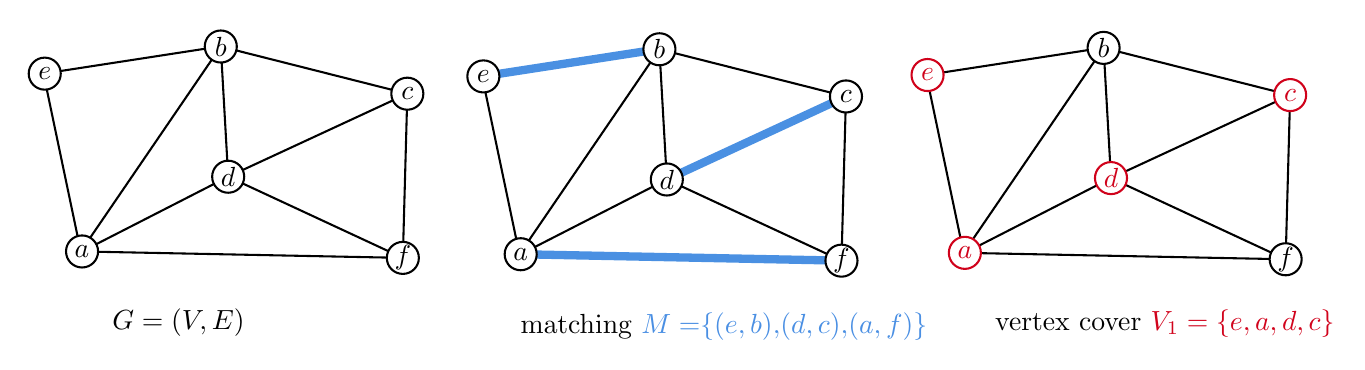
\begin{tikzpicture}[x=0.5pt,y=0.5pt,yscale=-1,xscale=1]
%uncomment if require: \path (0,237); %set diagram left start at 0, and has height of 237

%Straight Lines [id:da7485926733039977] 
\draw    (144.6,14.97) -- (43.43,163.09) ;
%Straight Lines [id:da4575120980127291] 
\draw [color={rgb, 255:red, 0; green, 0; blue, 0 }  ,draw opacity=1 ][line width=0.75]    (16.46,34.58) -- (143.69,14.97) ;
%Straight Lines [id:da9165715401778428] 
\draw    (16.46,34.58) -- (43.43,163.09) ;
%Straight Lines [id:da994182434786223] 
\draw [color={rgb, 255:red, 0; green, 0; blue, 0 }  ,draw opacity=1 ][line width=0.75]    (44.34,163.09) -- (276.17,167.73) ;
%Straight Lines [id:da9750224919648968] 
\draw    (149.95,109.07) -- (276.17,167.73) ;
%Straight Lines [id:da24348552449211425] 
\draw    (144.6,14.97) -- (149.95,109.07) ;
%Straight Lines [id:da16705340438790406] 
\draw    (144.6,14.97) -- (279.42,49.07) ;
%Straight Lines [id:da08663700279220432] 
\draw    (279.42,49.07) -- (276.17,167.73) ;
%Straight Lines [id:da16511775802360662] 
\draw [color={rgb, 255:red, 0; green, 0; blue, 0 }  ,draw opacity=1 ][line width=0.75]    (279.42,49.07) -- (149.95,109.07) ;
%Straight Lines [id:da4151454155794566] 
\draw    (149.95,109.07) -- (44.34,163.09) ;
%Shape: Ellipse [id:dp9133580928774087] 
\draw  [fill={rgb, 255:red, 255; green, 255; blue, 255 }  ,fill opacity=1 ] (5.79,34.58) .. controls (5.79,28.18) and (10.97,23) .. (17.37,23) .. controls (23.76,23) and (28.95,28.18) .. (28.95,34.58) .. controls (28.95,40.97) and (23.76,46.16) .. (17.37,46.16) .. controls (10.97,46.16) and (5.79,40.97) .. (5.79,34.58) -- cycle ;
%Shape: Ellipse [id:dp4005957609675306] 
\draw  [fill={rgb, 255:red, 255; green, 255; blue, 255 }  ,fill opacity=1 ] (133.02,14.97) .. controls (133.02,8.57) and (138.2,3.39) .. (144.6,3.39) .. controls (151,3.39) and (156.18,8.57) .. (156.18,14.97) .. controls (156.18,21.36) and (151,26.55) .. (144.6,26.55) .. controls (138.2,26.55) and (133.02,21.36) .. (133.02,14.97) -- cycle ;
%Shape: Ellipse [id:dp49214617921702164] 
\draw  [fill={rgb, 255:red, 255; green, 255; blue, 255 }  ,fill opacity=1 ] (267.84,49.07) .. controls (267.84,42.67) and (273.02,37.49) .. (279.42,37.49) .. controls (285.82,37.49) and (291,42.67) .. (291,49.07) .. controls (291,55.46) and (285.82,60.65) .. (279.42,60.65) .. controls (273.02,60.65) and (267.84,55.46) .. (267.84,49.07) -- cycle ;
%Shape: Ellipse [id:dp8440754424343925] 
\draw  [fill={rgb, 255:red, 255; green, 255; blue, 255 }  ,fill opacity=1 ] (138.37,109.07) .. controls (138.37,102.68) and (143.55,97.49) .. (149.95,97.49) .. controls (156.34,97.49) and (161.53,102.68) .. (161.53,109.07) .. controls (161.53,115.47) and (156.34,120.65) .. (149.95,120.65) .. controls (143.55,120.65) and (138.37,115.47) .. (138.37,109.07) -- cycle ;
%Shape: Ellipse [id:dp20660183368429152] 
\draw  [fill={rgb, 255:red, 255; green, 255; blue, 255 }  ,fill opacity=1 ] (32.76,163.09) .. controls (32.76,156.7) and (37.94,151.51) .. (44.34,151.51) .. controls (50.73,151.51) and (55.92,156.7) .. (55.92,163.09) .. controls (55.92,169.49) and (50.73,174.67) .. (44.34,174.67) .. controls (37.94,174.67) and (32.76,169.49) .. (32.76,163.09) -- cycle ;
%Shape: Ellipse [id:dp4098192910838151] 
\draw  [fill={rgb, 255:red, 255; green, 255; blue, 255 }  ,fill opacity=1 ] (264.59,167.73) .. controls (264.59,161.33) and (269.77,156.15) .. (276.17,156.15) .. controls (282.56,156.15) and (287.75,161.33) .. (287.75,167.73) .. controls (287.75,174.13) and (282.56,179.31) .. (276.17,179.31) .. controls (269.77,179.31) and (264.59,174.13) .. (264.59,167.73) -- cycle ;
%Straight Lines [id:da6233481480623783] 
\draw    (461.6,16.97) -- (360.43,165.09) ;
%Straight Lines [id:da9901942575404544] 
\draw [color={rgb, 255:red, 74; green, 144; blue, 226 }  ,draw opacity=1 ][line width=3]    (333.46,36.58) -- (460.69,16.97) ;
%Straight Lines [id:da3790939323014558] 
\draw    (333.46,36.58) -- (360.43,165.09) ;
%Straight Lines [id:da42115713644274366] 
\draw [color={rgb, 255:red, 74; green, 144; blue, 226 }  ,draw opacity=1 ][line width=3]    (361.34,165.09) -- (593.17,169.73) ;
%Straight Lines [id:da8702690824311631] 
\draw    (466.95,111.07) -- (593.17,169.73) ;
%Straight Lines [id:da34939805445985417] 
\draw    (461.6,16.97) -- (466.95,111.07) ;
%Straight Lines [id:da04544520748950576] 
\draw    (461.6,16.97) -- (596.42,51.07) ;
%Straight Lines [id:da5361594760285122] 
\draw    (596.42,51.07) -- (593.17,169.73) ;
%Straight Lines [id:da10465085418843478] 
\draw [color={rgb, 255:red, 74; green, 144; blue, 226 }  ,draw opacity=1 ][line width=3]    (596.42,51.07) -- (466.95,111.07) ;
%Straight Lines [id:da555393377892622] 
\draw    (466.95,111.07) -- (361.34,165.09) ;
%Shape: Ellipse [id:dp39324544068995604] 
\draw  [fill={rgb, 255:red, 255; green, 255; blue, 255 }  ,fill opacity=1 ] (322.79,36.58) .. controls (322.79,30.18) and (327.97,25) .. (334.37,25) .. controls (340.76,25) and (345.95,30.18) .. (345.95,36.58) .. controls (345.95,42.97) and (340.76,48.16) .. (334.37,48.16) .. controls (327.97,48.16) and (322.79,42.97) .. (322.79,36.58) -- cycle ;
%Shape: Ellipse [id:dp8663152391911655] 
\draw  [fill={rgb, 255:red, 255; green, 255; blue, 255 }  ,fill opacity=1 ] (450.02,16.97) .. controls (450.02,10.57) and (455.2,5.39) .. (461.6,5.39) .. controls (468,5.39) and (473.18,10.57) .. (473.18,16.97) .. controls (473.18,23.36) and (468,28.55) .. (461.6,28.55) .. controls (455.2,28.55) and (450.02,23.36) .. (450.02,16.97) -- cycle ;
%Shape: Ellipse [id:dp9564869279164044] 
\draw  [fill={rgb, 255:red, 255; green, 255; blue, 255 }  ,fill opacity=1 ] (584.84,51.07) .. controls (584.84,44.67) and (590.02,39.49) .. (596.42,39.49) .. controls (602.82,39.49) and (608,44.67) .. (608,51.07) .. controls (608,57.46) and (602.82,62.65) .. (596.42,62.65) .. controls (590.02,62.65) and (584.84,57.46) .. (584.84,51.07) -- cycle ;
%Shape: Ellipse [id:dp14244956479013948] 
\draw  [fill={rgb, 255:red, 255; green, 255; blue, 255 }  ,fill opacity=1 ] (455.37,111.07) .. controls (455.37,104.68) and (460.55,99.49) .. (466.95,99.49) .. controls (473.34,99.49) and (478.53,104.68) .. (478.53,111.07) .. controls (478.53,117.47) and (473.34,122.65) .. (466.95,122.65) .. controls (460.55,122.65) and (455.37,117.47) .. (455.37,111.07) -- cycle ;
%Shape: Ellipse [id:dp3916752397044988] 
\draw  [fill={rgb, 255:red, 255; green, 255; blue, 255 }  ,fill opacity=1 ] (349.76,165.09) .. controls (349.76,158.7) and (354.94,153.51) .. (361.34,153.51) .. controls (367.73,153.51) and (372.92,158.7) .. (372.92,165.09) .. controls (372.92,171.49) and (367.73,176.67) .. (361.34,176.67) .. controls (354.94,176.67) and (349.76,171.49) .. (349.76,165.09) -- cycle ;
%Shape: Ellipse [id:dp6775141746120102] 
\draw  [fill={rgb, 255:red, 255; green, 255; blue, 255 }  ,fill opacity=1 ] (581.59,169.73) .. controls (581.59,163.33) and (586.77,158.15) .. (593.17,158.15) .. controls (599.56,158.15) and (604.75,163.33) .. (604.75,169.73) .. controls (604.75,176.13) and (599.56,181.31) .. (593.17,181.31) .. controls (586.77,181.31) and (581.59,176.13) .. (581.59,169.73) -- cycle ;
%Straight Lines [id:da991028078692109] 
\draw    (782.6,15.97) -- (681.43,164.09) ;
%Straight Lines [id:da8020042074548936] 
\draw [color={rgb, 255:red, 0; green, 0; blue, 0 }  ,draw opacity=1 ][line width=0.75]    (654.46,35.58) -- (781.69,15.97) ;
%Straight Lines [id:da5410354625843318] 
\draw    (654.46,35.58) -- (681.43,164.09) ;
%Straight Lines [id:da1284005435452643] 
\draw [color={rgb, 255:red, 0; green, 0; blue, 0 }  ,draw opacity=1 ][line width=0.75]    (682.34,164.09) -- (914.17,168.73) ;
%Straight Lines [id:da4841445577516499] 
\draw    (787.95,110.07) -- (914.17,168.73) ;
%Straight Lines [id:da3189236797568633] 
\draw    (782.6,15.97) -- (787.95,110.07) ;
%Straight Lines [id:da24633327282247075] 
\draw    (782.6,15.97) -- (917.42,50.07) ;
%Straight Lines [id:da666695835406161] 
\draw    (917.42,50.07) -- (914.17,168.73) ;
%Straight Lines [id:da31804257401559455] 
\draw [color={rgb, 255:red, 0; green, 0; blue, 0 }  ,draw opacity=1 ][line width=0.75]    (917.42,50.07) -- (787.95,110.07) ;
%Straight Lines [id:da6699316806179542] 
\draw    (787.95,110.07) -- (682.34,164.09) ;
%Shape: Ellipse [id:dp818344887208882] 
\draw  [color={rgb, 255:red, 208; green, 2; blue, 27 }  ,draw opacity=1 ][fill={rgb, 255:red, 255; green, 255; blue, 255 }  ,fill opacity=1 ] (643.79,35.58) .. controls (643.79,29.18) and (648.97,24) .. (655.37,24) .. controls (661.76,24) and (666.95,29.18) .. (666.95,35.58) .. controls (666.95,41.97) and (661.76,47.16) .. (655.37,47.16) .. controls (648.97,47.16) and (643.79,41.97) .. (643.79,35.58) -- cycle ;
%Shape: Ellipse [id:dp5629283730413089] 
\draw  [fill={rgb, 255:red, 255; green, 255; blue, 255 }  ,fill opacity=1 ] (771.02,15.97) .. controls (771.02,9.57) and (776.2,4.39) .. (782.6,4.39) .. controls (789,4.39) and (794.18,9.57) .. (794.18,15.97) .. controls (794.18,22.36) and (789,27.55) .. (782.6,27.55) .. controls (776.2,27.55) and (771.02,22.36) .. (771.02,15.97) -- cycle ;
%Shape: Ellipse [id:dp21443256600205352] 
\draw  [color={rgb, 255:red, 208; green, 2; blue, 27 }  ,draw opacity=1 ][fill={rgb, 255:red, 255; green, 255; blue, 255 }  ,fill opacity=1 ] (905.84,50.07) .. controls (905.84,43.67) and (911.02,38.49) .. (917.42,38.49) .. controls (923.82,38.49) and (929,43.67) .. (929,50.07) .. controls (929,56.46) and (923.82,61.65) .. (917.42,61.65) .. controls (911.02,61.65) and (905.84,56.46) .. (905.84,50.07) -- cycle ;
%Shape: Ellipse [id:dp17023173827913307] 
\draw  [color={rgb, 255:red, 208; green, 2; blue, 27 }  ,draw opacity=1 ][fill={rgb, 255:red, 255; green, 255; blue, 255 }  ,fill opacity=1 ] (776.37,110.07) .. controls (776.37,103.68) and (781.55,98.49) .. (787.95,98.49) .. controls (794.34,98.49) and (799.53,103.68) .. (799.53,110.07) .. controls (799.53,116.47) and (794.34,121.65) .. (787.95,121.65) .. controls (781.55,121.65) and (776.37,116.47) .. (776.37,110.07) -- cycle ;
%Shape: Ellipse [id:dp21431691922786544] 
\draw  [color={rgb, 255:red, 208; green, 2; blue, 27 }  ,draw opacity=1 ][fill={rgb, 255:red, 255; green, 255; blue, 255 }  ,fill opacity=1 ] (670.76,164.09) .. controls (670.76,157.7) and (675.94,152.51) .. (682.34,152.51) .. controls (688.73,152.51) and (693.92,157.7) .. (693.92,164.09) .. controls (693.92,170.49) and (688.73,175.67) .. (682.34,175.67) .. controls (675.94,175.67) and (670.76,170.49) .. (670.76,164.09) -- cycle ;
%Shape: Ellipse [id:dp6777828112816564] 
\draw  [fill={rgb, 255:red, 255; green, 255; blue, 255 }  ,fill opacity=1 ] (902.59,168.73) .. controls (902.59,162.33) and (907.77,157.15) .. (914.17,157.15) .. controls (920.56,157.15) and (925.75,162.33) .. (925.75,168.73) .. controls (925.75,175.13) and (920.56,180.31) .. (914.17,180.31) .. controls (907.77,180.31) and (902.59,175.13) .. (902.59,168.73) -- cycle ;

% Text Node
\draw (17.37,34.58) node   [align=left] {$\displaystyle e$};
% Text Node
\draw (144.6,14.97) node   [align=left] {$\displaystyle b$};
% Text Node
\draw (279.42,49.07) node   [align=left] {$\displaystyle c$};
% Text Node
\draw (149.95,109.07) node   [align=left] {$\displaystyle d$};
% Text Node
\draw (44.34,163.09) node   [align=left] {$\displaystyle a$};
% Text Node
\draw (276.17,167.73) node   [align=left] {$\displaystyle f$};
% Text Node
\draw (64,202) node [anchor=north west][inner sep=0.75pt]   [align=left] {$\displaystyle G=( V,E)$};
% Text Node
\draw (334.37,36.58) node   [align=left] {$\displaystyle e$};
% Text Node
\draw (461.6,16.97) node   [align=left] {$\displaystyle b$};
% Text Node
\draw (596.42,51.07) node   [align=left] {$\displaystyle c$};
% Text Node
\draw (466.95,111.07) node   [align=left] {$\displaystyle d$};
% Text Node
\draw (361.34,165.09) node   [align=left] {$\displaystyle a$};
% Text Node
\draw (593.17,169.73) node   [align=left] {$\displaystyle f$};
% Text Node
\draw (359,205) node [anchor=north west][inner sep=0.75pt]   [align=left] {matching $\displaystyle \textcolor[rgb]{0.29,0.56,0.89}{M=}\textcolor[rgb]{0.29,0.56,0.89}{\{}\textcolor[rgb]{0.29,0.56,0.89}{(}\textcolor[rgb]{0.29,0.56,0.89}{e,b}\textcolor[rgb]{0.29,0.56,0.89}{)}\textcolor[rgb]{0.29,0.56,0.89}{,}\textcolor[rgb]{0.29,0.56,0.89}{(}\textcolor[rgb]{0.29,0.56,0.89}{d,c}\textcolor[rgb]{0.29,0.56,0.89}{)}\textcolor[rgb]{0.29,0.56,0.89}{,}\textcolor[rgb]{0.29,0.56,0.89}{(}\textcolor[rgb]{0.29,0.56,0.89}{a,f}\textcolor[rgb]{0.29,0.56,0.89}{)}\textcolor[rgb]{0.29,0.56,0.89}{\}}$};
% Text Node
\draw (655.37,35.58) node  [color={rgb, 255:red, 208; green, 2; blue, 27 }  ,opacity=1 ] [align=left] {$\displaystyle e$};
% Text Node
\draw (782.6,15.97) node   [align=left] {$\displaystyle b$};
% Text Node
\draw (917.42,50.07) node  [color={rgb, 255:red, 208; green, 2; blue, 27 }  ,opacity=1 ] [align=left] {$\displaystyle c$};
% Text Node
\draw (787.95,110.07) node  [color={rgb, 255:red, 208; green, 2; blue, 27 }  ,opacity=1 ] [align=left] {$\displaystyle d$};
% Text Node
\draw (682.34,164.09) node  [color={rgb, 255:red, 208; green, 2; blue, 27 }  ,opacity=1 ] [align=left] {$\displaystyle a$};
% Text Node
\draw (914.17,168.73) node   [align=left] {$\displaystyle f$};
% Text Node
\draw (702,203) node [anchor=north west][inner sep=0.75pt]   [align=left] {vertex cover $\displaystyle \textcolor[rgb]{0.82,0.01,0.11}{V_{1} =\{e,a,d,c\}}$};


\end{tikzpicture}

